\documentclass[aps,prl,twocolumn,superscriptaddress,footinbib]{revtex4-1}
\usepackage[utf8]{inputenc}
\usepackage[colorlinks=true,linkcolor=cyan,citecolor=cyan,urlcolor=cyan]{hyperref}
\usepackage{bm,bbm,amssymb,amsmath}
\usepackage{graphicx}
\usepackage[dvipsnames]{xcolor}

\newcommand{\Msun}{\ensuremath{\,M_{\odot}}}
\newcommand{\apjl}{Astrophys. J. Lett.}

\newcommand{\FZU}{CEICO, FZU-Institute of Physics of the Czech Academy of Sciences,
Na Slovance 1999/2, 182 21 Prague 8, Czech Republic}
\newcommand{\CITA}{Canadian Institute for Theoretical Astrophysics, University of Toronto, Toronto, Ontario M5S 3H8, Canada}

\begin{document}

\title{Prospects for constraining twin stars with next-generation \\ gravitational-wave detectors}

\author{Philippe Landry}
\affiliation{\CITA}
\email{plandry@cita.utoronto.ca}
\author{Kabir Chakravarti}
\affiliation{\FZU}
\email{chakravarti@fzu.cz}

\begin{abstract}
Neutron star equations of state with strong phase transitions may support twin stars, hybrid and hadronic stars with the same mass but different tidal deformabilities.
The presence of twins in the population of merging neutron stars produces distinctive gaps in the joint distribution of binary tidal deformabilities and chirp masses.
We analyze a simulated population of binary neutron star mergers recovered with a network of next-generation (XG) gravitational-wave detectors to determine how many observations are needed to infer, or rule out, the existence of twin stars. Using a hierarchical inference framework based on a simple parametric twin-star model, we find that a single week of XG observations may suffice to detect a tidal deformability difference of several hundred between twins and measure the mass scale at which twins occur to within a few percent. For less pronounced twins, XG observations will place a stringent upper bound on the tidal deformability difference.
\end{abstract}

\maketitle

\paragraph{Introduction.}

The phase structure of matter at the highest densities realized inside neutron stars (NSs) is an unsolved puzzle for nuclear physics. Above the nuclear saturation density of $\rho_{\rm nuc} = 2.8\times 10^{14}$ g/cm$^3$, the nucleonic constituents of ordinary matter are thought to give way to other fundamental degrees of freedom, such as hyperons or deconfined quarks. If this phase transition occurs at a density that prevails inside NSs, then the heaviest of these compact objects may in fact be hybrid stars with exotic-matter cores. The possible existence of a stable family of hybrid stars with central densities greater than those of conventional hadronic NSs has been envisioned and studied extensively from the theoretical point of view~\cite{Gerlach1968, Kampfer1981, GlendenningKettner2000, SchertlerGreiner2000, AlfordHan2013, ZdunikHaensel2013, BenicBlaschke2015, AlfordBurgio2015, HanSteiner2019}.

In many nuclear theory models, the transition to the high-density phase is of first order, exhibiting a discontinuous first derivative of the baryon chemical potential with respect to baryon density $\rho$. The hadronic- and exotic-matter phases may either remain separate and interface directly, or they may be linked by an intermediate mixed phase. In the former scenario, the so-called Maxwell construction, the baryon density experiences a discontinuity $\Delta\rho$ at fixed pressure $p$.  
If $\Delta\rho$ is sufficiently large, the dense matter equation of state (EOS) may support stable twin stars: hadronic- and hybrid-star counterparts with the same mass, but different compactness~\cite{Schaffner-BielichHanauske2002, ZacchiTolos2017, AlfordSedrakian2017, ChristianZacchi2018}.

\begin{figure}[htb]
    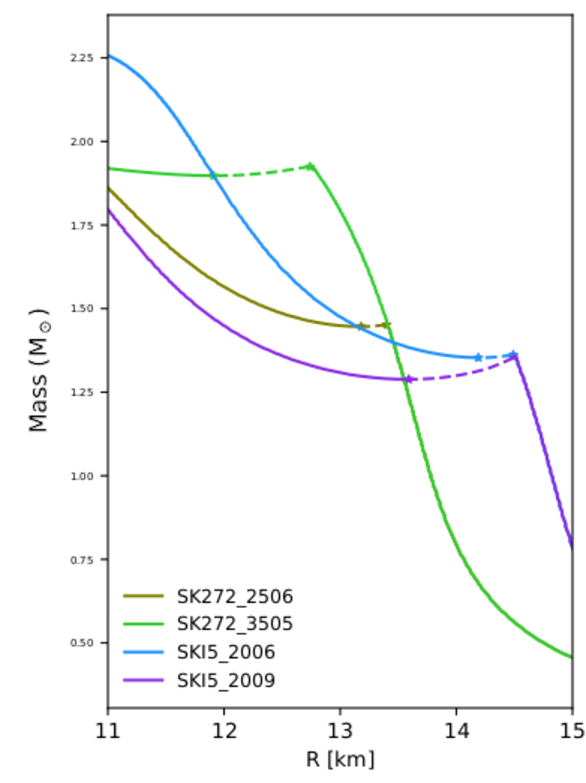
\includegraphics[width=0.47\columnwidth,trim={5 5 1 2},clip]{M-R.pdf} 
    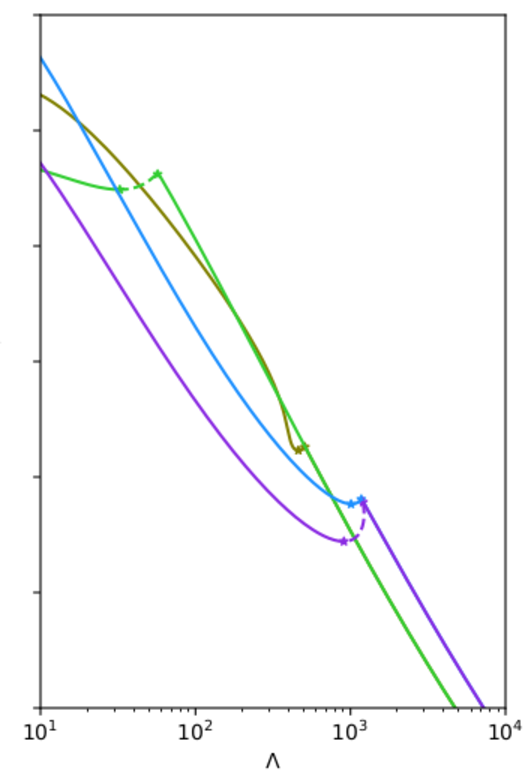
\includegraphics[width=0.43\columnwidth,trim={2 5 1 3},clip]{M-L.pdf}
    \caption{Sequences of neutron star properties for selected twin-star-supporting equations of state. We plot the mass-radius (left) and mass-tidal deformability (right) relations. Dashed lines indicate unstable segments where no neutron stars exist. Markers bookend the twin-star mass range.}
    \label{fig:twins}
\end{figure}

Such twin-star configurations are visible in Fig.~\ref{fig:twins}'s mass-radius ($m$--$R$) and mass-tidal deformability ($m$--$\Lambda$) relations for selected EOSs. The presence of radius or tidal deformability twins is a smoking gun for the occurrence of a strong first-order phase transition inside NSs.

Because twin stars provide such a clear signature, their compatibility with existing observations of NSs has been heavily scrutinized. Parametric EOSs supporting twin stars have been constructed~\cite{PaschalidisYagi2018,MontanaTolos2019,ChristianZacchi2019,PangDietrich2020,WangShi2022} to simultaneously satisfy observational constraints on the tidal deformability from the compact binary merger GW170817~\cite{GW170817,LVC_GW170817source,LVC_GW170817eos} and bounds on the maximum mass $M_{\rm TOV}$ from the heaviest pulsars discovered in radio surveys~\cite{AntoniadisFreire2013,CromartieFonseca2020,FonsecaCromartie2021}. Reference~\cite{ChristianSchaffner-Bielich2020} argued that the radius measured for PSR J0030+0451 via X-ray pulse profile modeling~\cite{RileyWatts2019,MillerLamb2019} rules out twin stars associated with a phase transition below $1.7\rho_{\rm nuc}$. Twin stars were also shown~\cite{ChristianSchaffner-Bielich2022} to be compatible with the inferred radius of PSR J0740+6620~\cite{RileyWatts2021,MillerLamb2021} and~\cite{LiSedrakian2021} with PREX-II's measurement of the neutron skin of $^{208}$Pb~\cite{AdhikariAlbataineh2021}. Meanwhile, Ref.~\cite{ChristianSchaffner-Bielich2021_Mmax} suggested (contra Ref.~\cite{TsaloukidisKoliogiannis2022}) that a maximum mass in excess of $2.2\Msun$ might exclude twin stars across the entire NS mass spectrum. Hence, although existing astronomical observations substantially restrict the parameter space for twin stars, they remain a live possibility.

Additional observations of NSs with the existing gravitational-wave (GW) detector network of Advanced LIGO~\cite{aLIGO}, Virgo~\cite{aVirgo} and KAGRA~\cite{AkutsuAndo2021} could, in principle, turn up a serendipitous discovery of twin stars. However, this is unlikely given the typically narrow mass range over which twins are supported and the high resolution in $\Lambda$ required to identify them---not to mention the modest expected binary neutron star (BNS) detection rate~\cite{AbbottAbbott2018_ObservingScenarios,ColomboSalafia2022,PatricelliBernardini2022}.
Prospects for detecting twin stars with next-generation (XG) ground-based GW observatories like Cosmic Explorer~\cite{EvansAdhikari2021} and Einstein Telescope~\cite{MaggioreVanDenBroeck2020} are more promising, thanks to their ability to capture virtually the complete merging NS population in the nearby Universe~\cite{EvansAdhikari2021,BorhanianSathyaprakash2022}. Although precisely measuring the tidal deformability of individual NSs will remain a challenging task \footnote{Ref.~\cite{SmithBorhanian2021} reports statistical uncertainties of $O(100\%)$ in component tidal deformabilities even for a simulated XG BNS merger at 40 Mpc with signal-to-noise ratio 2400.}, twin-star-supporting EOSs give rise to a distinctive distribution of binary tidal deformabilities $\tilde{\Lambda}$ vs chirp masses $\mathcal{M}$ across the population~\cite{ChatziioannouHan2020}: as shown in Fig.~\ref{fig:lambdapop}, the distribution is contiguous when no twin stars are present, whereas twins introduce gaps that make it disjoint. This population-level signature can be used to infer the existence of twin stars even when individual twin-star pairs are not identifiable. Here we show that XG measurements of the binary tidal deformability distribution can detect the existence of twin stars at 90\% confidence (or with a log Bayes factor greater than 6) with as few as $\sim 100$ observations.

To do so, we first construct a family of EOSs with first-order phase transitions giving rise to stable twins, and simulate populations of BNS mergers recovered with different GW detector networks. We then collect the binary tidal deformability and chirp mass measurements from each population. Heuristically, twin stars are detected at the population level when the recovered distribution is disjoint, rather than contiguous. To implement this test systematically, we develop a Bayesian hierarchical inference framework with a parametric model for the $m$--$\Lambda$ relation, formulated in terms of a twin-star mass scale $M_t$ and the tidal deformability difference $\Delta\Lambda$ between twins. This approach follows Ref.~\cite{ChatziioannouHan2020}, which tackled the related problem of inferring the radius difference between hybrid and hadronic stars with LIGO and Virgo.
We find that current GW detectors, even at upgraded ``A+'' sensitivities~\cite{AbbottAbbott2018_ObservingScenarios}, cannot meaningfully constrain the twin-star parameters. However, in the best-case scenario we consider, an XG network can determine $M_t$ and $\Delta\Lambda$ to within 1\% and 15\%, respectively, at 90\% confidence after just one month of observations.

\begin{figure}[t]
    \centering
    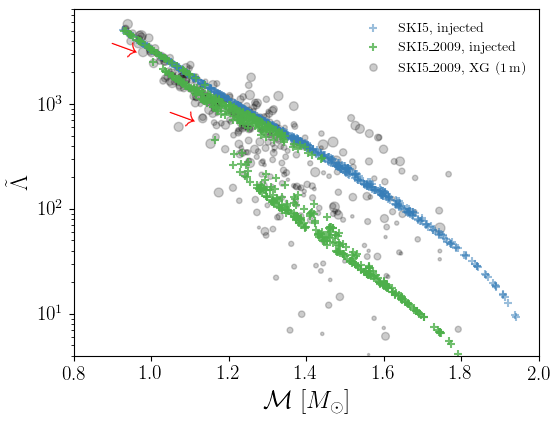
\includegraphics[width=0.9\columnwidth,trim={5 5 5 5},clip]{SKI52009_pop.png}
    \caption{Joint binary tidal deformability and chirp mass distribution probed by one month of XG observations for the twin-star-supporting SKI5\_2009 equation of state, as compared with the purely hadronic SKI5 equation of state. A uniform neutron star mass distribution is assumed. The gaps in the distribution for SKI5\_2009, indicated by the arrows, signify the existence of twin stars (cf.~the contiguous SKI5 distribution). The detected distribution is subject to statistical uncertainties and is scattered by detector noise; for SKI5\_2009, we show the recovered chirp masses and binary tidal deformabilities in grey, with marker sizes inversely proportional to the signal-to-noise ratio. Actual statistical uncertainties are $O(10^2)$ in $\tilde{\Lambda}$ and $O(10^{-3})$ in $\mathcal{M}$.}
    \label{fig:lambdapop}
\end{figure}

\paragraph{Tidal deformability distribution.}\label{Sec_BNSPop}
To determine when twin stars are identifiable in the BNS population, we generate simulated distributions of masses and binary tidal deformabilities. We prescribe a NS mass model, select an EOS, sample a realization of the astrophysical population of BNS mergers, and determine which events are detected by computing their optimal signal-to-noise ratio (SNR) with respect to the detector network of interest.

The EOSs we adopt are constructed using the constant-sound-speed formulation of Ref.~\cite{HanSteiner2019}, in which a constant-pressure phase transition segment of length (or ``strength'') $\Delta\rho$ and onset density $\rho_t$ interpolates between a low-density hadronic EOS and a causal high-density extension. We vary the hadronic EOS and the phase transition parameters to explore the parameter space that is compatible with existing NS observations. The resulting set of EOSs is displayed in Fig.~\ref{fig:twins}.

Our fiducial NS mass distribution is uniform for $m \in [1\Msun,M_{\rm TOV}]$, with random pairing into binaries.
The binary tidal deformability for each BNS is determined from its masses by the $m$--$\Lambda$ relation dictated by the EOS. Neutron stars in the twin-star mass range are randomly assigned to the hadronic or the hybrid branch of the relation with equal probability. 

We sample from this population and determine the subset of mergers that are detected in three different detector networks: the ``HLV'' network includes LIGO-Hanford, LIGO-Livingston and Virgo detectors at their design sensitivities; the ``A+'' network upgrades the LIGO-Hanford and LIGO-Livingston detectors to A+ sensitivity; and the ``XG'' network replaces the LIGO detectors with Cosmic Explorer detectors, and the Virgo detector with Einstein Telescope, at their respective design sensitivities. Given our assumed distribution of sources and merger rate of 440 Gpc$^{-3}$ y$^{-1}$~\cite{LVK_O3bPop}, our simulated populations yield expected astrophysical rates of 3, 15 and 5800 BNS mergers per year within the sensitive ranges~\cite{AbbottAbbott2018_ObservingScenarios} for HLV, A+ and XG, respectively. The exact number of detections depends on the population realization, but the detection efficiency is $\sim60\%$ for A+ and $\sim95\%$ for XG. Since the HLV network makes so few detections, we focus our analysis on the A+ and XG scenarios. For each detected event, we simulate the GW likelihood as a multivariate Gaussian with a covariance that scales inversely with SNR.

An example of the resulting observed distribution of binary tidal deformabilities vs chirp masses is illustrated in Fig.~\ref{fig:lambdapop} for SKI5\_2009. One can clearly see the disjoint nature of the true, underlying distribution, but it is less visible when the data is scattered by detector noise. For EOSs with smaller $\Delta\Lambda$, the gaps in the distribution may not be discernible by eye at all. 
The need to simultaneously account for statistical uncertainty in the masses and tidal deformabilities of individual events, as well as uncertainty in the underlying $m$--$\Lambda$ relation, motivates the hierarchical inference framework we describe below.

\paragraph{Hierarchical inference.}\label{Sec_inference}

We systematically search for evidence of twin stars in the binary tidal deformability vs chirp mass distribution using a simple model. We prescribe a parametric population model

\begin{equation}
    \pi(\mathcal{M},q,\tilde{\Lambda}|\boldsymbol{\theta},\boldsymbol{\lambda}) = \pi(\tilde{\Lambda}|\mathcal{M},q;\boldsymbol{\theta}) \pi(\mathcal{M},q|\boldsymbol{\lambda})
\end{equation}
built from a binary tidal deformability distribution

\begin{align} \label{lambdadist}
    \pi(\tilde{\Lambda}|\mathcal{M},q;\boldsymbol{\theta}) = \int& P(\tilde{\Lambda}|\Lambda_1,\Lambda_2,q) \pi(\Lambda_1|m_1;\boldsymbol{\theta}) \pi(\Lambda_2|m_2;\boldsymbol{\theta}) \nonumber \\ 
    &\times P(m_1,m_2|\mathcal{M},q) d\Lambda_1 d\Lambda_2 dm_1 dm_2 
\end{align}
that depends on parameters $\boldsymbol{\theta}$ describing an $m$--$\Lambda$ relation $\pi(\Lambda|m;\boldsymbol{\theta}) = \delta(\Lambda - \Lambda_{\boldsymbol{\theta}}(m))$, and a mass distribution

\begin{equation}
    \pi(\mathcal{M},q;\boldsymbol{\lambda}) = \int P(\mathcal{M},q|m_1,m_2) \pi(m_1,m_2|\boldsymbol{\lambda}) dm_1 dm_2
\end{equation}
that depends on parameters $\boldsymbol{\lambda}$, expressed here in terms of a joint distribution $\pi(m_1,m_2|\boldsymbol{\lambda})$ for the component masses $m_{1,2}$. A hierarchical inference of the population model parameters $\boldsymbol{\theta}, \boldsymbol{\lambda}$ proceeds according to~\cite{MandelFarr2019}

\begin{align} \label{bayes}
    P(\boldsymbol{d}|\boldsymbol{\theta},\boldsymbol{\lambda}) = \prod_i \frac{1}{\zeta(\boldsymbol{\theta},\boldsymbol{\lambda})} \int& P(d_i | \mathcal{M},q,\tilde{\Lambda}) \nonumber \\ 
    &\times \pi(\mathcal{M},q,\tilde{\Lambda} | \boldsymbol{\theta},\boldsymbol{\lambda}) \,d\mathcal{M}\, dq\, d\tilde{\Lambda} ,
\end{align}
where $P(d_i|\mathcal{M},q,\tilde{\Lambda})$ is the marginal GW likelihood in chirp mass, mass ratio and binary tidal deformability for the $i$th observation, and $\zeta(\boldsymbol{\theta},\boldsymbol{\lambda})$ is the fraction of the population that is detected. Since we are only interested in the $m$--$\Lambda$ relation parameters $\boldsymbol{\theta}$ in our application, we fix the mass distribution as specified above. We also ignore selection effects, as they do not impact the recovery of the parameters of interest: in our population model, the detection fraction is approximately independent of the EOS \footnote{The GW selection function for BNS mergers is proportional to $\mathcal{M}^{5/2}$~\cite{ChatziioannouFarr2020}, so the detection fraction depends on the EOS via the maximum mass in the population, set here by $M_{\rm TOV}$. However, $M_{\rm TOV}$ varies by only $\sim10\%$ across the chosen EOSs.}.
Thus, we approximate Eq.~\eqref{bayes} as
\begin{equation}
    P(\boldsymbol{d}|\boldsymbol{\theta}) \propto \prod_i \int P(d_i | \mathcal{M},q,\tilde{\Lambda}) \, \pi(\mathcal{M},q,\tilde{\Lambda} | \boldsymbol{\theta}) \, d\mathcal{M} \, dq \, d\tilde{\Lambda} .
\end{equation}
We adopt uniform priors on the parameters $\boldsymbol{\theta}$, such that the posterior $P(\boldsymbol{\theta}|\boldsymbol{d})$ is proportional to this expression.

To evaluate the likelihood $P(\boldsymbol{d}|\boldsymbol{\theta})$, we make a Monte Carlo approximation for the integrals over $\mathcal{M}$ and $q$. The remaining integral is resolved by the delta function in $\tilde{\Lambda}$ that results from Eq.~\eqref{lambdadist}. We then have

\begin{equation}
    P(\boldsymbol{d}|\boldsymbol{\theta}) \approx \prod_i \sum_j P(d_i | \mathcal{M}_j,q_j,\tilde{\Lambda}_{\boldsymbol{\theta}}(\mathcal{M}_j,q_j)) \; | \; \mathcal{M}_j, q_j \sim \pi(\mathcal{M},q)
\end{equation}
modulo normalization. We sample from this likelihood using a Markov-chain Monte Carlo algorithm implemented with \texttt{emcee}~\cite{Foreman-MackeyHogg2013}.

To model the twin-star $m$--$\Lambda$ relations, we adopt the parametric form

\begin{widetext}
\begin{equation}
    \Lambda_{\boldsymbol{\theta}} = \begin{cases} \Lambda_{1.4}^{\rm had} \left(m/1.4 \Msun\right)^{-6} & 1\Msun \leq m \leq M_t \\
    \left[\Lambda_{1.4}^{\rm had} \left(M_t/1.4 \Msun\right)^{-6} - \Delta\Lambda\right] \left[\left(\frac{m}{M_t}\right)^{-k} - \frac{(1-m/M_t)}{(1-M_{\rm TOV}/M_t)} \left(\frac{M_{\rm TOV}}{M_t}\right)^{-k}\right] +\Lambda_{\rm TOV} \frac{(1-m/M_t)}{(1-M_{\rm TOV}/M_t)} & M_t < m \leq M_{\rm TOV} \\
    \end{cases}
\label{fit}
\end{equation}
\end{widetext}
with parameters $\boldsymbol{\theta} = \lbrace \Lambda_{1.4}^{\rm had}, M_{t}, \Delta\Lambda, k, M_{\rm TOV}, \Lambda_{\rm TOV} \rbrace$, i.e.~the tidal deformability of a canonical hadronic NS, the (median) twin-star mass, the tidal deformability difference between twins of mass $M_t$, the power-law slope of $\Lambda(m)$ on the hybrid branch, the maximum NS mass and the tidal deformability of the maximum-mass star, respectively. To keep the model simple, we do not model the finite extent of the twin star mass range; $M_{t}$ simply represents its midpoint. Thus, the twin-star signature that informs the hierarchical inference is the existence of a gap of width $\Delta\Lambda$ in the tidal deformability distribution at $M_{t}$, rather than the multimodality of the tidal deformability distribution itself. This model for the $m$--$\Lambda$ relation is shown in Fig.~\ref{fig:diagram}.

The uniform priors for the $m$--$\Lambda$ relation parameters are subjected to the constraints $1.00\Msun \leq M_{t} \leq 1.94\Msun$, $0 \leq \Delta\Lambda \leq 1500$, $5 \leq k \leq 12$. Finding that $\Lambda_{1.4}$ is always well-recovered, and that the results are relatively insensitive to the maximum-mass parameters, we fix $M_{\rm TOV}$, $\Lambda_{1.4}$ and $\Lambda_{\rm TOV} = 3$ for simplicity.

\begin{figure}[b]
    \centering
    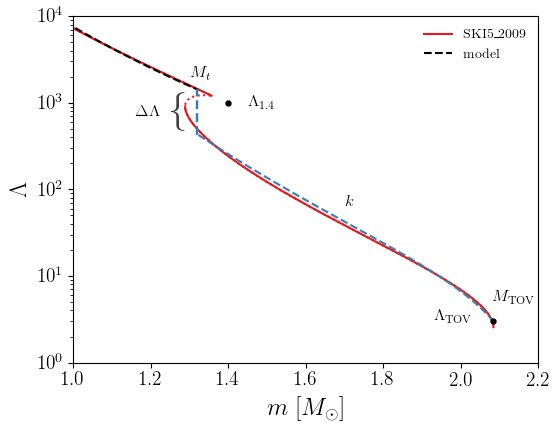
\includegraphics[width=0.9\columnwidth,trim={5 5 5 5},clip]{SKI52009_fit.png}
    \caption{Parametric model for the mass-tidal deformability relation used in the hierarchical inference. We show the fit for SKI5\_2009 and highlight the parameters we infer in blue.}
    \label{fig:diagram}
\end{figure}

\paragraph{Results.}\label{Sec_res}

We apply the hierarchical inference of twin-star parameters to the populations simulated for the hybrid EOSs displayed in Fig.~\ref{fig:twins}, as well as the purely hadronic EOSs SKI5 and SK272. For the hadronic cases, we expect to recover the prior on $M_{t}$ and a posterior peaked at $\Delta\Lambda = 0$. For the other cases, we expect to recover a posterior on $\Delta\Lambda$ peaked away from zero, and a constraint on $M_{t}$. We consider the twin stars as detected if the marginal $\Delta\Lambda$ highest-posterior-density interval excludes zero at 90\% confidence. As an alternative quantification of the evidence for twin stars, we also compute an evidence ratio (Bayes factor) between the hypotheses that twin stars are present and absent in the population.

\begin{figure*}[t]
    \centering
    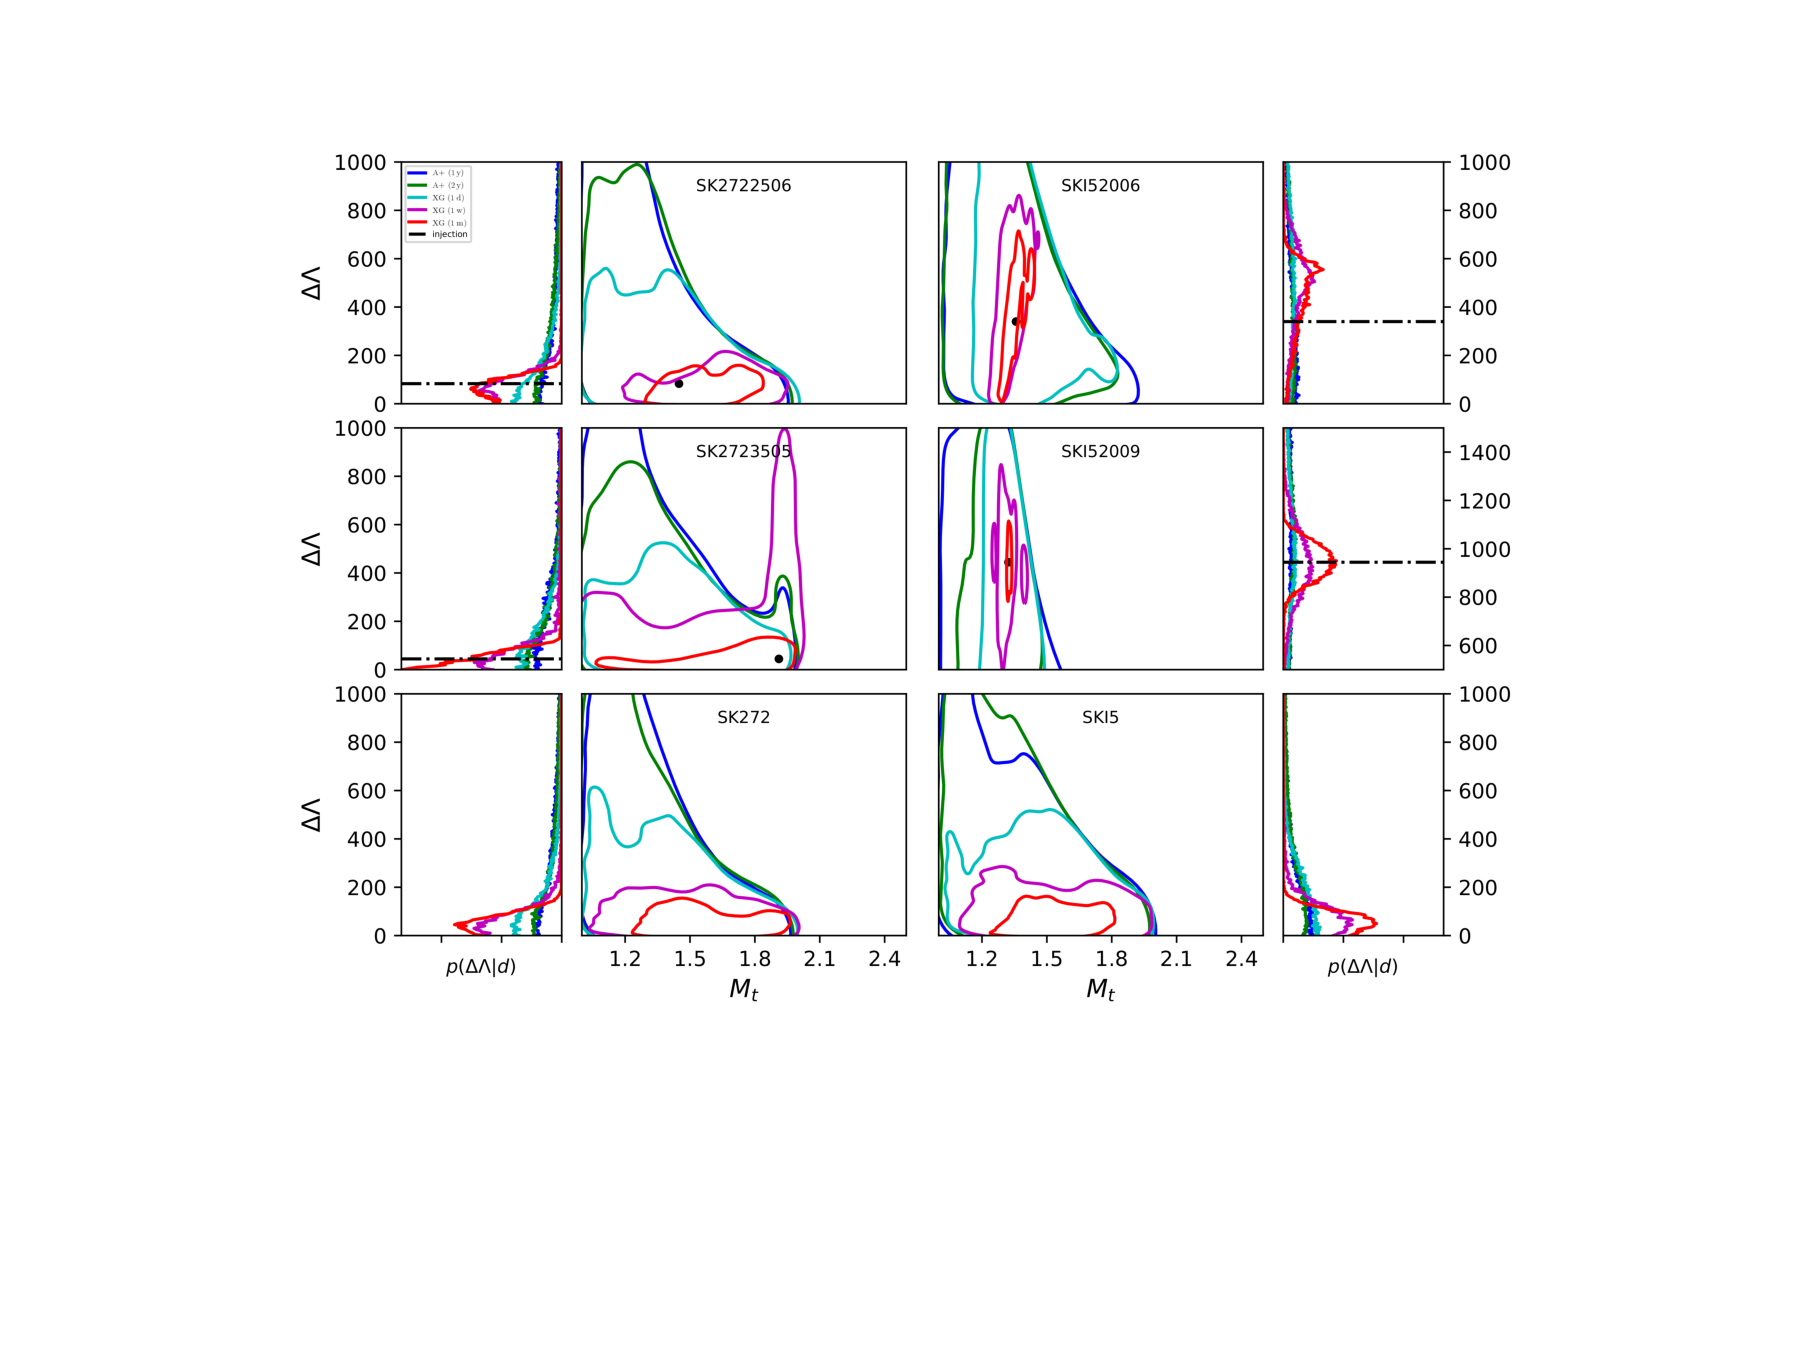
\includegraphics[width=0.83\textwidth,trim={145 168 135 74},clip]{unif-moneyplot.pdf}
    \caption{Posteriors on twin-star parameters of the mass-tidal deformability relation for different equations of state. The 90\% credible region of the posterior, averaged over 10 population realizations, is shown for various observing scenarios. The parameters corresponding to the injected equation of state are indicated in black; in the bottom two panels, where the injected equation of state is purely hadronic, the $M_t$ parameter has no intrinsic meaning.}
    \label{fig:results}
\end{figure*}

The recovered twin star parameters for each EOS are shown in Fig.~\ref{fig:results} for a sequence of observing scenarios, from one year at A+ sensitivity to one month at XG sensitivity. We show the average recovery over 10 population realizations to mitigate statistical fluctuations in the confidence regions. 
For the EOS with the strongest phase transition, SKI5\_2009, the one-dimensional marginal posterior on $\Delta\Lambda$ already comfortably favors the presence of twin stars at 90\% confidence after one week of observation with the XG network. The $\Delta\Lambda$ posterior for SKI5\_2006, which has the same onset density but a weaker phase transition, also satisfies our twin-star detection criterion after one week of XG observations.

For the EOSs with higher onset densities, and correspondingly smaller $\Delta\Lambda$, the tidal deformability resolution in the XG observations is not sufficient to distinguish between zero and finite $\Delta\Lambda$. However, after one month of XG observations, $\Delta\Lambda \gtrsim 100$ can be ruled out at 90\% confidence for both SK272\_2506 and SK272\_3505. This resolution limit also holds for the recoveries of the hadronic EOSs SKI5 and SK272: the $\Delta\Lambda$ posteriors converge towards zero as expected, but cannot exclude $\Delta\Lambda \lesssim 100$.

Thus, after one month of XG observations, we correctly conclude that twin stars are present in the BNS populations for SKI5\_2009 and SKI5\_2006, and that twin stars with $\Delta\Lambda \gtrsim 100$ are excluded in the other scenarios.
Meanwhile, the $\Delta\Lambda$ posteriors after even two years of A+ observations are essentially uninformative in all cases.

The evidence ratios between twin and no-twin hypotheses tell a similar story. For each EOS and observing scenario, we compute the Bayes factor $B$ as a Savage-Dickey density ratio~\cite{Dickey1971}, the ratio of marginal posterior to marginal prior at $\Delta\Lambda = 0$, obtaining the former via a kernel density estimate. We plot the evolution of the Bayes factors in  Fig.~\ref{fig:bfs} as a function of the number of BNS mergers detected within a redshift $z < 0.5$; the error bands quantify the variation in $B$ over 10 population realizations. As can be seen, for SKI5\_2009 the evidence is decidedly in favor of twin stars ($\log{B} < -6$) after a week of XG observations ($\sim100$ detections). For SKI5\_2006, the evidence favors twin stars more modestly ($\log{B} \approx -3$), although some population realizations yield as decisive a result as for SKI5\_2009. For the other four cases, the Bayes factor favors the no-twins hypothesis only moderately ($\log{B} \approx 3$) even after a month of XG observations ($\sim500$ detections). This reinforces the conclusion that an XG network can confidently detect $\Delta\Lambda \gtrsim 100$, but is resolution-limited for smaller $\Delta\Lambda$.

Having established the prospects for twin star detection, we now investigate how well the twin-star parameters can be measured. The main panels of Fig.~\ref{fig:results} relate the accuracy and precision with which $\Delta\Lambda$ and $M_t$ are recovered. 
We find that the recoveries are accurate at 90\% confidence for all of the EOSs we study. However, for SKI5\_2009, the mode of the posterior slightly overestimates the tidal deformability difference. We attribute this to the very small range $\Delta M_t \approx 0.01\Msun$ over which this EOS supports twin stars, which means that the gaps in the tidal deformability distribution are easily mimicked by statistical fluctuations in the data. For SKI272\_3505, the posterior mode instead slightly underestimates $M_t$, which we attribute to the proximity between $M_t$ and $M_{\rm TOV}$ for this EOS.  
For the hadronic EOSs SKI5 and SK272, the $M_t$ parameter is meaningless, and we observe that the recovered value tends to be close to the midpoint of the NS mass spectrum. 

Overall, we find that $M_t$ is more precisely constrained than $\Delta\Lambda$. In the best-case scenario, for SKI5\_2009, $M_t$ and $\Delta\Lambda$ are determined to within 1\% and 15\% uncertainty, respectively, after one month of observation. In contrast, after two years of A+ observations, the uncertainties are respectively 15\% and 68\%. Even in our most pessimistic scenario, for SK272\_3505, $M_t$ and $\Delta\Lambda$ are measured with respective errors of 20\% and 150\% after one month at XG sensitivity. 

\paragraph{Discussion.}

Our investigations demonstrate how hierarchical inference on a population of BNS mergers can be used to systematically test for the presence of twin stars. We find that an XG network is needed to definitively identify (or rule out) twin stars with GWs at the population level, and that this may be accomplished with as little as one week of observation. An XG network can resolve a tidal deformability difference between twins of several hundred, and constrain the twin-star mass scale to within a few percent. When realized in future, measurements of this kind will guide the development of nuclear theory models for the NS EOS.

Although the parametric $m$--$\Lambda$ relation model we adopt is deliberately kept simple, our results indicate that it will suffice for accurate twin-star parameter measurements into the XG era. Nonetheless, when future observing campaigns return thousands of BNS detections, it may be desirable to use a more sophisticated model that represents the finite extent of the twin-star mass range more faithfully, or to parameterize the $m$--$\Lambda$ relation in terms of microscopic quantities that are more directly informative for nuclear theory.  
The general method laid out here can be adapted straightforwardly to accommodate these modifications. It would also work to detect other phenomena giving rise to ostensible twins, e.g.~an overlap in the NS and black hole mass spectra or a separate family of stellar-mass exotic compact objects.

\begin{figure}[hb]
    \centering
    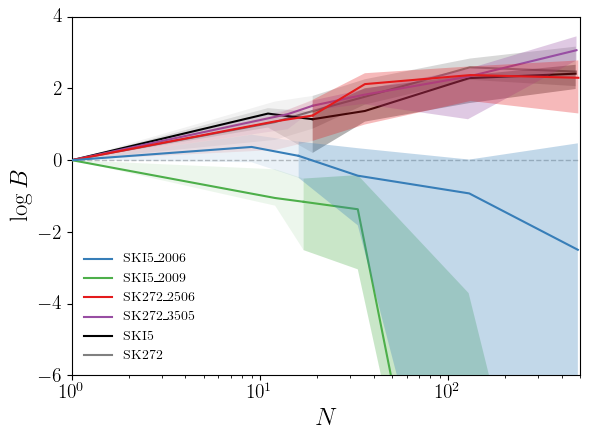
\includegraphics[width=0.9\columnwidth,trim={5 10 5 5},clip]{BFs.png}
    \caption{Model comparison between twin-star and no-twin hypotheses for each injected equation of state. We show how the log Bayes factor evolves as a function of the number of observations in the A+ era (light shading) and the XG era (dark shading). A negative $\log B$ favors the presence of twin stars. The shaded regions encompass 68\% confidence intervals on $\log B$  due to its variation across 10 population realizations.}
    \label{fig:bfs}
\end{figure}

\acknowledgments

The authors thank Katerina Chatziioannou and Jolien Creighton for useful suggestions about this work.
P.L. is supported by the Natural Sciences \& Engineering Research Council of Canada (NSERC).
K.C. is supported by the Czech Academy of Sciences under the project number LQ100102101.
The authors are grateful for computational resources provided by the LIGO Lab and supported by NSF Grants PHY-0757058 and PHY-0823459.

\bibliographystyle{apsrev4-1}
\bibliography{references}

\end{document}
